%%%%%%%%%%%%%%%%%%%%%%%%
%
% $Autor: Wings $
% $Datum: 2020-07-24 09:05:07Z $
% $Pfad: GDV/Vortraege/latex - Ausarbeitung/Kapitel/Einleitung.tex $
% $Version: 4732 $
%
%%%%%%%%%%%%%%%%%%%%%%%%

\chapter{Introduction}

\section{Introduction}

The focus of this analysis is to identify and mitigate potential threats and weaknesses within Orgadata’s SimplyTag system. SimplyTag facilitates quick access to construction-related data through a web app, making it essential to safeguard against malicious actors attempting to exploit the system. This involves analyzing logs to detect suspicious activity and ensure data integrity.

\section{Challenges and Results}

\begin{figure}
	\begin{center}
		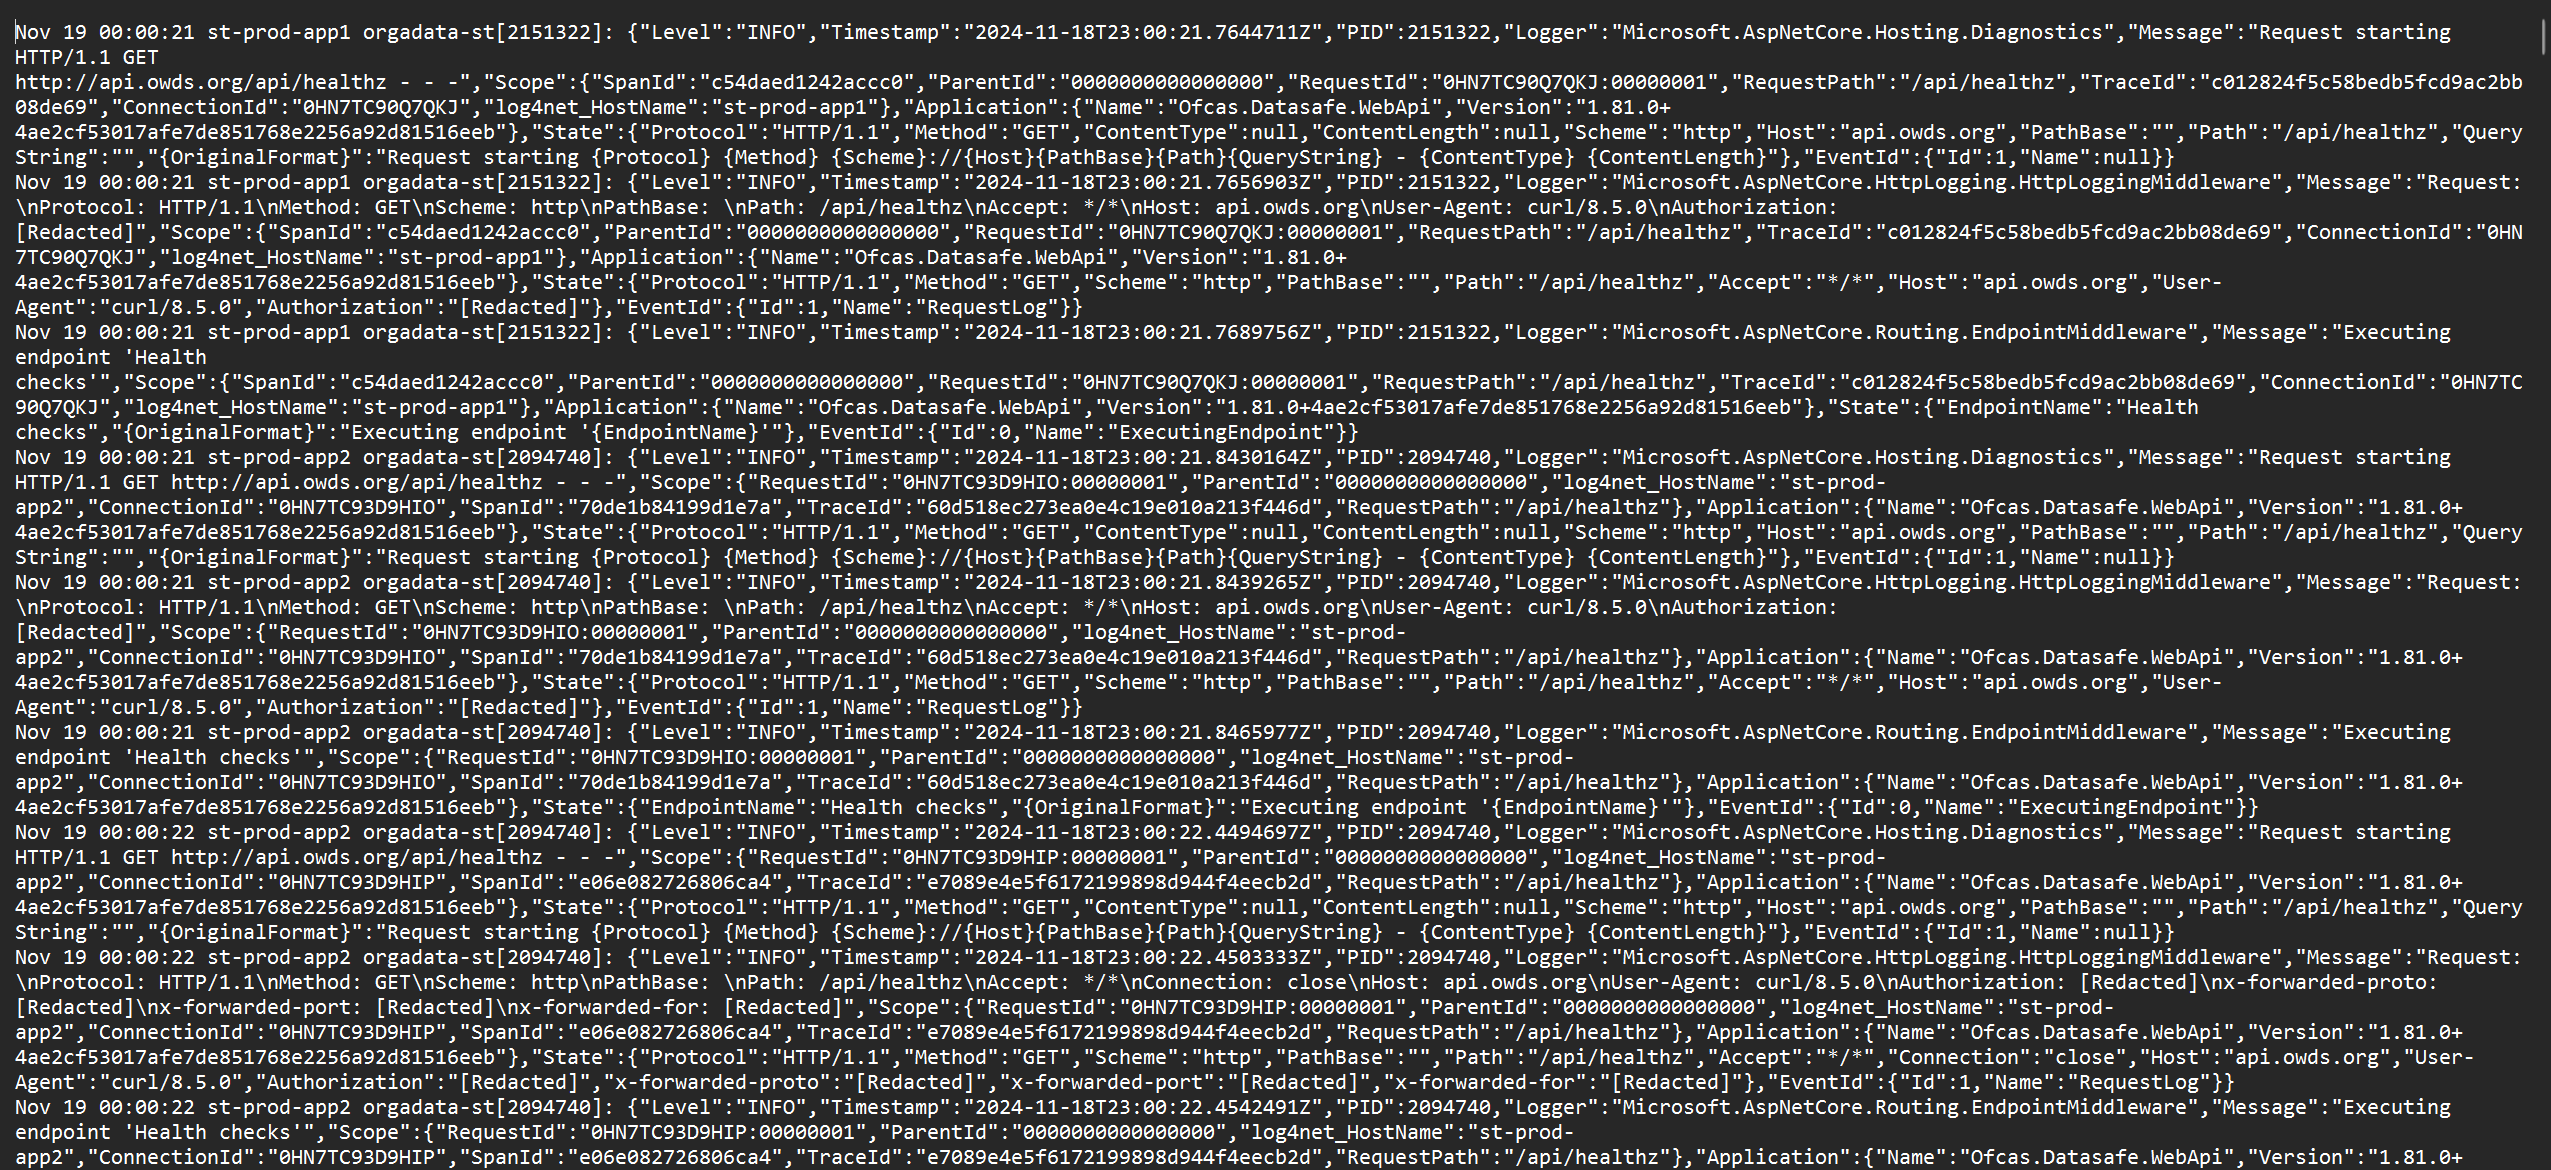
\includegraphics[width=0.7\linewidth]{Images/Data_Img.png}
		\caption{Original Data format}
		\label{Data_Img} 
	\end{center}
\end{figure}

\textbf{Challenges:}
\begin{itemize}
	\item Handling large-scale logs to pinpoint anomalies as shown in the figure ~\ref{Data_Img}.
	\item Differentiating legitimate user activity from malicious attempts.
	\item Establishing efficient protocols to respond to detected threats.
\end{itemize}

\textbf{Results Achieved:}
\begin{itemize}
	\item Implementation of enhanced monitoring protocols using trace IDs and HTTP status codes.
	\item Reduced data breaches by identifying and blocking unauthorized requests.
\end{itemize}



